\documentclass[11pt,a4paper,fleqn]{article}
\usepackage[T1]{fontenc}
\usepackage[utf8]{inputenc}
\usepackage[british]{babel}
\usepackage{lmodern}
\usepackage[margin=2.3cm]{geometry}
\usepackage{amsmath,amssymb,bm}
\usepackage{textcomp}
\usepackage{xcolor}
\usepackage{tikz}
\usetikzlibrary{arrows.meta,calc,positioning,shapes.geometric}
\usepackage{tcolorbox}
\usepackage{booktabs}
\usepackage{array}
\usepackage{tabularx}
\usepackage{multicol}
\usepackage{enumitem}
\usepackage{etoolbox}
\usepackage[font=small,labelfont=bf,hypcap=false]{caption}
\usepackage[colorlinks=true,linkcolor=black,citecolor=blue!50!black,urlcolor=blue!50!black]{hyperref}
\usepackage{parskip}
\usepackage[compact]{titlesec}
\titlespacing*{\section}{0pt}{2.0ex plus .6ex minus .4ex}{0.8ex plus .2ex}
\titlespacing*{\subsection}{0pt}{1.4ex plus .5ex minus .3ex}{0.4ex plus .2ex}
\usepackage{fancyhdr}
\setlength{\headheight}{14pt}
\pagestyle{fancy}
\fancyhf{}
\lhead{\small DeCAF --- Drill Tracking: Problem and Proposed Estimator}
\rhead{\small As of 13 November 2026}
\cfoot{\thepage}
\setlist[itemize]{leftmargin=*, itemsep=2pt, parsep=0pt, topsep=2pt}
\setlist[enumerate]{leftmargin=*, itemsep=2pt, parsep=0pt, topsep=2pt}
\emergencystretch=2em
\widowpenalty=10000
\clubpenalty=10000
% compact two-column bibliography (heading outside the columns)
\patchcmd{\thebibliography}{\section*{\refname}}{}{}{}
\apptocmd{\thebibliography}{\setlength{\itemsep}{0.5pt}\setlength{\parsep}{0pt}}{}{}

\newtcolorbox{mybox}[1]{colback=red!5!white,colframe=red!75!black,fonttitle=\bfseries,title={#1}}

% notation as in the thesis (Methods 3.3.7, 3.4)
\newcommand{\Tcm}{\mathbf{T}_{\mathrm{cm}}}
\newcommand{\Ptd}{\mathbf{P}^{\mathrm{tip}}_{\mathrm{d}}}
\newcommand{\Ptc}{\mathbf{P}^{\mathrm{tip}}_{\mathrm{c}}}
\newcommand{\stip}{\sigma_{\mathrm{tip}}}

\begin{document}

\begin{center}
  {\LARGE Drill Tracking: Problem and Proposed Estimator}\\[2mm]
  {\large Why the drawn drill tip jumps today, and how an estimator with memory fixes it}\\[2mm]
  {\small DeCAF --- Master's thesis \quad$\cdot$\quad As of 13 November 2026}
\end{center}

\begin{mybox}{Summary}
\begin{itemize}[leftmargin=*, itemsep=1pt, topsep=0pt]
  \item Today the pose of the drill is computed anew in every camera frame; nothing is averaged over time.
  \item Each frame either draws the \emph{fused pose} (colour corners plus IR points) or, if one of four checks
        fails, the \emph{colour pose} plus a frozen offset from the last fused frame (\emph{carry}).
  \item The colour pose is weak in depth and its error changes from frame to frame, so the frozen offset only fits
        the frame it was taken from: the tip jumps even with the drill at rest (lab test on 11 Nov: \textbf{83 jumps
        larger than 5\,mm}).
  \item The new estimator replaces the switching by \emph{one} iterated Kalman filter: it remembers the last pose,
        uses all colour corners and IR points of every frame weighted by their reliability, and down-weights
        outliers instead of discarding the IR points of whole frames.
  \item With the drill clamped, the tip jitter on the test data drops from \textbf{0.657 to 0.215\,mm}, i.e.\ to
        about one third.
  \item It does not remove the constant offset of about 1.5--2\,mm between tip and reference that exists today.
  \item It is built into the C++ tracking engine and on by default in the live display; switched off,
        computation and display are as before (13 Nov 2026).
\end{itemize}
\end{mybox}

Derivations, all settings and the exact conditions of each number are in the German report
\emph{Bohrer-Tracking: Problem und neuer Schätzer} in the same folder.

%==========================================================================================
\section{How Tracking Works Today}
\label{sec:today}

\begin{itemize}
  \item \textbf{Input.} Every cycle the camera delivers a colour image and, with a tool loaded, an image pair of the
        two IR cameras. The C++ tracking engine computes the \emph{pose} of the drill, i.e.\ where the cylinder
        marker lies and how it is rotated.
  \item \textbf{Tip.} The tip $\mathbf{P}^{\mathrm{tip}}$ is a point rigidly attached to the marker,
        \textbf{179.36\,mm} from the marker origin.
  \item \textbf{1 Colour pose.} The engine finds the checkerboard corners of the marker in the colour image, matches
        them to the model corners and computes the \emph{colour pose}. A small filter per corner smooths the corner
        positions slightly; the pose itself is not smoothed.
  \item \textbf{2 IR points and fused pose.} The same corners are searched in both IR images; a corner found in both
        gives a 3D point by triangulation (an \emph{IR point}). From colour corners and IR points together the
        engine computes the \emph{fused pose}. The colour pose is uncertain in depth (along the camera's line of
        sight) and in the tilt of the cylinder; the IR points carry their own depth, so the fused pose is much
        better determined in these directions.
  \item \textbf{3 Four checks.} Four yes/no checks decide for the whole frame whether the fused pose is used: at
        least 6 IR points; IR points fit the model (residual at most 2.5\,mm); fused pose moves the marker origin
        at most 6\,mm away from the colour pose; fused pose does not fit the colour image clearly worse than the
        colour pose.
  \item \textbf{4 Drawing.} If the checks pass, the fused pose is drawn (\emph{fused} frames) and the offset between
        fused tip and colour tip is stored. Otherwise the colour pose is drawn, usually plus the stored offset if it
        is at most 1\,s old (\emph{carry} frames). The offset is frozen: it does not rotate with the drill and ends
        abruptly after 1\,s.
  \item \textbf{Initial guess.} The engine refines the colour pose from an initial guess that always comes from the
        colour pose of the previous frame, never from the fused pose (dashed loop in Fig.~\ref{fig:today}). The
        better depth of the fused pose therefore never helps the next frame.
  \item \textbf{Analogy.} Two kitchen scales: one weighs accurately, the other is off by an amount that depends on
        where the parcel lies. Switching between them and adding a once-measured difference to the second one still
        makes the reading jump, because that difference was only right once. Fused pose = accurate scale, colour pose
        = inaccurate scale, carry offset = once-measured difference.
\end{itemize}

\begin{figure}[!htb]
\centering
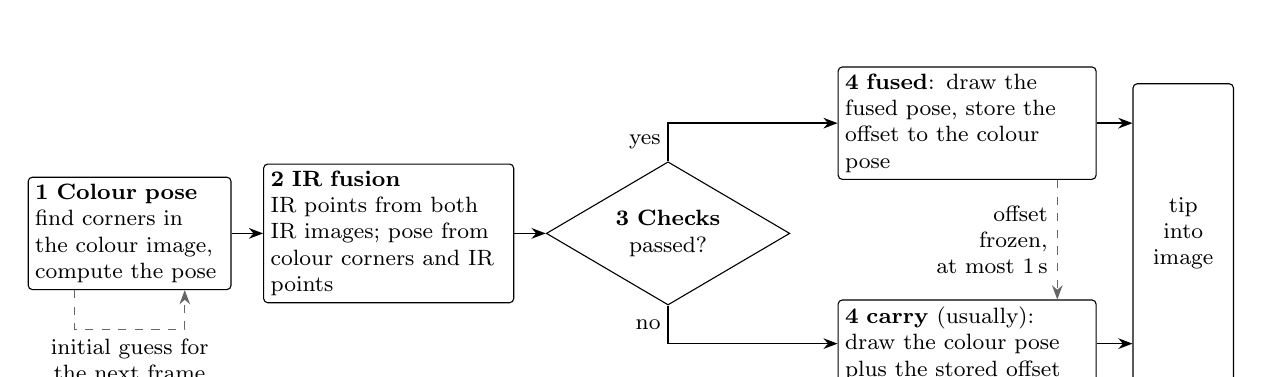
\begin{tikzpicture}[
  font=\footnotesize,
  box/.style={draw, rounded corners=1.5pt, align=left, inner sep=2.5pt, fill=white, text width=#1,
              execute at begin node={\hyphenpenalty=10000\exhyphenpenalty=10000}},
  box/.default=26mm,
  dec/.style={draw, diamond, aspect=1.7, align=center, inner sep=0pt, text width=21mm,
              execute at begin node={\hyphenpenalty=10000\exhyphenpenalty=10000}},
  arr/.style={-{Stealth[length=1.8mm]}, semithick},
  fb/.style={-{Stealth[length=1.8mm]}, dashed, black!60},
  lab/.style={font=\footnotesize, fill=white, inner sep=1pt, align=center}
]
\node[box=24mm] (F) at (0,0) {\textbf{1 Colour pose}\\ find corners in the colour image, compute the pose};
\node[box=30mm, right=4mm of F] (I) {\textbf{2 IR fusion}\\ IR points from both IR images; pose from colour corners
and IR points};
\node[dec, right=4mm of I] (D) {\textbf{3 Checks}\\ passed?};
\node[box=31mm, anchor=west] (FU) at ($(D.east)+(6mm,14mm)$) {\textbf{4 fused}: draw the fused pose, store the
offset to the colour pose};
\node[box=31mm, anchor=west] (CA) at ($(D.east)+(6mm,-14mm)$) {\textbf{4 carry} (usually): draw the colour pose plus
the stored offset};
\node[draw, rounded corners=1.5pt, fill=white, align=center, text width=11mm, inner sep=2.5pt,
      minimum height=38mm] (Z) at ($(FU.east)!0.5!(CA.east)+(11mm,0)$) {tip\\ into\\ image};
\draw[arr] (F) -- (I);
\draw[arr] (I) -- (D);
\draw[arr] (D.north) |- node[lab, pos=0.25, left=0.5mm] {yes} (FU.west);
\draw[arr] (D.south) |- node[lab, pos=0.25, left=0.5mm] {no} (CA.west);
\draw[arr] (FU.east) -- (FU.east -| Z.west);
\draw[arr] (CA.east) -- (CA.east -| Z.west);
\draw[fb] ([xshift=-5mm]FU.south east) -- node[lab, left=0.8mm, align=right, fill=none, text=black] {offset\\ frozen,\\ at most 1\,s} ([xshift=-5mm]CA.north east);
\draw[fb] ([xshift=-7mm]F.south) -- ++(0,-5mm) -| ([xshift=7mm]F.south);
\node[lab, anchor=north, align=center] at ($(F.south)+(0,-5.8mm)$) {initial guess for\\ the next frame};
\end{tikzpicture}
\caption{Today's processing per camera frame, simplified. Depending on the checks, either the fused pose from colour
corners and IR points is drawn (fused) or the colour pose, usually plus the frozen offset of the last fused frame
(carry). Without a stored offset the plain colour pose is drawn. The initial guess for the next frame always comes
from the colour pose; the pose is not averaged over time.}
\label{fig:today}
\end{figure}

%==========================================================================================
\section{What Goes Wrong}
\label{sec:problem}

\textbf{Data.} Recordings with raw images that can be replayed through the tracking offline, mostly with the tip in
a seat of the calibration board; the seat position from the measured board pose is the \emph{reference}. Split into
\emph{tuning data} and \emph{test data}; plus the live log of the lab test on 11 Nov (no raw images).
\emph{Jitter} = RMS of the tip around its mean in a recording (a constant offset to the reference does not count);
\emph{jump} = tip distance between two consecutively drawn frames.

\subsection*{(a) Every Frame Stands Alone \textnormal{(fine jitter)}}
\begin{itemize}
  \item The previous frame only provides the initial guess and a comparison for plausibility checks; the noise of
        each frame passes almost unfiltered to the tip.
  \item The long lever of 179.36\,mm magnifies every small tilt error of the marker at the tip
        \cite[pp.~535, 543]{west2004designing}; that per-frame pose estimates jitter is well known in tracking
        \cite[pp.~60--61, 72]{lepetit2005monocular}, \cite[Sec.~III.A]{vacchetti2004stable}.
  \item Measured: with the drill clamped, today's tip jitters with \textbf{0.657\,mm} on the test data.
  \item At rest one could average over many frames; this is not done. Rest is common at the patient, e.g.\ with the
        drill at the entry point.
\end{itemize}

\subsection*{(b) Switching Between Two Estimates \textnormal{(large jumps)}}
\begin{itemize}
  \item Each frame decides anew which pose is drawn; every switch can make the tip jump by the difference of the
        two poses. The carry offset only compensates this difference for the frame it was taken from.
  \item Lab test on 11 Nov, drill at rest (corner motion median 0.41\,px per frame): of 2063 frames with a new pose,
        286 (13.9\,\%) were carry frames, mostly single ones between fused frames.
  \item The tip jumped \textbf{83 times by more than 5\,mm}, 75 of them at a switch between fused and carry, at
        most by 12.84\,mm.
  \item The carry tip lay 3.67\,mm (median) from the typical fused tip, almost only along the camera's line of
        sight, i.e.\ exactly in the depth direction where the colour pose is weak.
  \item Small, flat-looking targets often have two nearly equally good pose solutions, and the pose then jumps even
        in a static scene \cite[pp.~2024, 2029]{schweighofer2006robust}, \cite[pp.~5772, 5775]{jin2017sensor}
        (only an analogy; not checked for this marker). Such an error is not noise and cannot be fixed by sending
        finished poses through a Kalman filter \cite[Sec.~I]{liu2021navigation}; a prior that already acts on the
        feature level can help \cite[Sec.~III-D]{liu2021navigation}.
\end{itemize}

\subsection*{(c) A Check Discards the IR Points When They Would Help Most \textnormal{(large jumps)}}
\begin{itemize}
  \item One check rejects the fusion if the fused pose moves the marker origin more than 6\,mm away from the colour
        pose. It measures the error of the colour pose, not the quality of the IR data: the worse the colour pose,
        the more the fusion has to correct, and the more likely it is rejected.
  \item Lab test: on all carry frames 32--50 IR points were available, mostly fitting the model well (residual median
        0.81\,mm); on \textbf{78.7\,\%} of the carry frames the 6-mm check was the only reason for the rejection.
  \item A rejection discards \emph{all} IR points of the frame. Real measurements rarely split cleanly into inliers
        and outliers \cite[p.~308]{triggs2000bundle}; continuous robust weighting is the usual alternative to binary
        thresholds \cite[Sec.~II]{kerl2013robust}, \cite[§9.3--9.4]{zhang1997parameter}.
  \item \textbf{How (b) and (c) acted together.} The marker sat at the top left image border (about 600\,px from the
        image centre, blurred, with colour fringes), so the colour pose was poor. The 6-mm check sorted the frames:
        where the colour pose was close, the fusion was accepted and the offset stored (colour origin 2.53\,mm from
        the fused one, median); where it was far off, carry was drawn (colour origin 6.8\,mm from its typical fused
        position, median). The offset from a good frame was applied to a bad frame, and the tip jumped.
\end{itemize}

\subsection*{(d) Uncertain First Frame, No Uncertainty in the Display}
\begin{itemize}
  \item Right after \emph{locking on} (first detection of the marker after start or loss) there is no stored offset.
        If the fusion is not accepted on that frame, the plain colour pose is drawn.
  \item With the drill clamped, the largest deviation of today's tip from its mean occurred on such a first frame
        with the plain colour pose, in tuning and test data alike (test data: \textbf{6.07\,mm}).
  \item The display does not know how certain the tip is; there is no uncertainty in millimetres live. The only
        warning is orange instead of green when less than 75\,\% of the marker is visible. The tip appears exact,
        which is what Simpson et al.\ criticise in navigation displays \cite{simpson2014computation}.
\end{itemize}

%==========================================================================================
\section{The New Estimator}
\label{sec:new}

\begin{itemize}
  \item \textbf{What it is.} One new last stage behind the engine's existing pose computation; settings and pose
        computation of the engine stay unchanged. Technically an \emph{iterated Kalman filter}: every frame it
        combines a prediction from earlier frames with the new measurements, each weighted by its reliability, and
        refines the result in three small steps (Fig.~\ref{fig:step}).
  \item \textbf{Memory (fixes a).} The prediction for the new frame is the pose of the last frame (random walk
        \cite[Ex.~4.1, 4.2]{saerkkae2013bayesian}); its uncertainty grows each frame, only little at rest. At rest
        each new frame moves the estimate only a little, which acts like an average over many frames. Assumption,
        not yet checked: very fast free motion is unlikely at the patient.
  \item \textbf{One result instead of two (fixes b).} No switching between two estimates. Each measurement pulls the
        pose as far as its reliability justifies; a frame without IR points is carried by the prediction and the
        colour corners instead of by a frozen offset. Working on the individual measurements is called tight
        coupling, as opposed to filtering finished poses \cite[p.~493]{tobergte2009robust}; colour and stereo
        measurements in one covariance-weighted Huber cost are used in ORB-SLAM2
        \cite[Sec.~III-C]{murartal2017orbslam2}.
  \item \textbf{All measurements, weighted by reliability.} Every frame uses all colour corners and, except in the
        cases below, all IR points, each with its own uncertainty. The IR uncertainty is narrow across the IR ray
        and wide along it, like the triangulation error \cite[§II]{matthies1987error}. How reliable both kinds of
        measurement are was scaled from the observed residuals with the tip at rest (robust median scale
        \cite[Eq.~(28)]{zhang1997parameter}).
  \item \textbf{Down-weight instead of discard (fixes c).} The worse a measurement fits the joint solution, the lower
        its weight (Huber weighting, iteratively reweighted least squares \cite[§9.4]{zhang1997parameter}). The
        6-mm distance check no longer decides whether IR points are used, so exactly the frames that fail it today
        keep their IR points. IR points of a frame are only left out if there are fewer than 6, or if they fit the
        model grossly badly (residual above 6\,mm; same quantity as today's 2.5-mm check, not a distance check).
  \item \textbf{Follows real motion.} If the marker corners move together in the image, the prediction becomes more
        uncertain and the estimate follows the measurements. The principle (smooth strongly at rest, open with
        motion) is known from the 1\,€ filter \cite{casiez2012oneeuro} and from instrument tracking
        \cite[pp.~279--280]{cai2024distributed}; the concrete opening is our own heuristic, tuned on the tuning data.
  \item \textbf{Knows its uncertainty (fixes d).} The pose comes with its covariance, propagated to the tip in
        millimetres \cite[Eq.~55]{sola2018micro}. Also on the first frame after locking on, colour corners and IR
        points are used together. After locking on, the tip stays hidden until its uncertainty is at most 2\,mm,
        for at most 5 frames (about 167\,ms).
  \item \textbf{Starting point.} Each frame the computation starts at the pose the engine outputs (fused if the
        checks pass, otherwise colour). It does not change the engine's own initial guess for the colour pose.
        After a gap or an engine reset the estimator starts again without memory.
\end{itemize}

\begin{figure}[!htb]
\centering
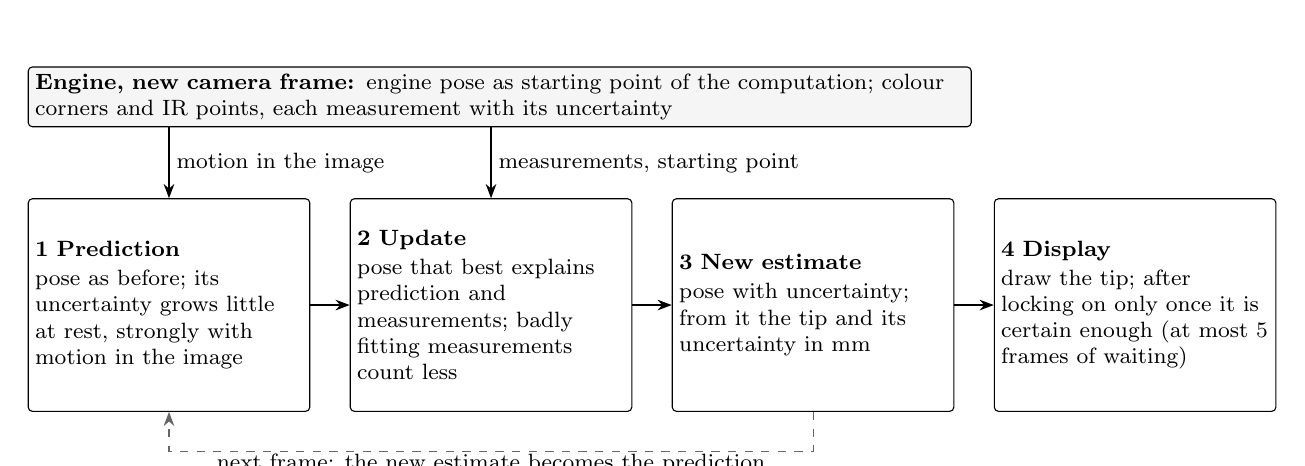
\begin{tikzpicture}[
  font=\footnotesize,
  st/.style={draw, rounded corners=1.5pt, align=left, text width=34mm, minimum height=27mm, inner sep=2.5pt,
             fill=white, execute at begin node={\hyphenpenalty=10000\exhyphenpenalty=10000}},
  inp/.style={draw, rounded corners=1.5pt, align=left, inner sep=2.5pt, fill=black!4,
              execute at begin node={\hyphenpenalty=10000\exhyphenpenalty=10000}},
  arr/.style={-{Stealth[length=1.8mm]}, semithick},
  fb/.style={-{Stealth[length=1.8mm]}, dashed, black!60},
  lab/.style={font=\footnotesize, fill=white, inner sep=1pt}
]
\node[st] (V) at (0,0) {\textbf{1 Prediction}\\[1pt] pose as before; its uncertainty grows little at rest, strongly
with motion in the image};
\node[st, right=5mm of V] (U) {\textbf{2 Update}\\[1pt] pose that best explains prediction and measurements; badly
fitting measurements count less};
\node[st, right=5mm of U] (P) {\textbf{3 New estimate}\\[1pt] pose with uncertainty; from it the tip and its
uncertainty in mm};
\node[st, right=5mm of P] (A) {\textbf{4 Display}\\[1pt] draw the tip; after locking on only once it is certain
enough (at most 5 frames of waiting)};
\node[inp, text width=118mm, anchor=south west] (E) at ($(V.north west)+(0,9mm)$)
  {\textbf{Engine, new camera frame:} engine pose as starting point of the computation; colour corners and IR
   points, each measurement with its uncertainty};
\draw[arr] (V) -- (U);
\draw[arr] (U) -- (P);
\draw[arr] (P) -- (A);
\draw[arr] (E.south -| V) -- node[lab, right=0.5mm] {motion in the image} (V.north);
\draw[arr] (E.south -| U) -- node[lab, right=0.5mm] {measurements, starting point} (U.north);
\draw[fb] (P.south) -- ++(0,-5mm) -| (V.south);
\node[lab, anchor=north] at ($(V.south)!0.5!(P.south)+(0,-5mm)$) {next frame: the new estimate becomes the
prediction};
\end{tikzpicture}
\caption{One step of the new estimator. The estimate of the last frame becomes the prediction for the new frame; the
update combines it with the measurements of the new frame, each according to its reliability. After locking on, i.e.\
the first detection of the marker after start or loss, there is no prediction yet, and only the measurements
count.}
\label{fig:step}
\end{figure}

\begin{mybox}{For the interested reader: what is computed per frame}
State: the pose $\mathbf{x}_k = \Tcm$ (marker $\to$ colour camera) with covariance $\boldsymbol{\Sigma}_k$.
Prediction: $\bar{\mathbf{x}}_k = \hat{\mathbf{x}}_{k-1}$, $\bar{\boldsymbol{\Sigma}}_k = \boldsymbol{\Sigma}_{k-1}
+ \mathbf{Q}_k$ ($\mathbf{Q}_k$ small at rest, large with image motion). Update:
\begin{equation*}
  \hat{\mathbf{x}}_k = \arg\min_{\mathbf{x}}\;
  \tfrac12\,\bigl\lVert \mathbf{x} \boxminus \bar{\mathbf{x}}_k \bigr\rVert^2_{\bar{\boldsymbol{\Sigma}}_k^{-1}}
  + \sum_i \rho(e_i) + \sum_j \rho(e_j),
\end{equation*}
with $e_i$, $e_j$ the normalised residuals of colour corner $i$ (image) and IR point $j$ (space) and $\rho$ the Huber
function (quadratic up to $c = 1.5$, linear above). Pose composition and covariance on
$\mathrm{T}(3)\times\mathrm{SO}(3)$ as in \cite[Ex.~7, Eqs.~51--52]{sola2018micro}. Solved with three
Gauss--Newton steps from the engine pose, re-weighting each time. Without $\rho$ the iterated Kalman update is
Gauss--Newton on this cost \cite{bell1993iterated}, \cite[p.~30]{lepetit2005monocular}, i.e.\ a local MAP estimate
\cite[§4.2.5--4.2.6]{barfoot2017state}; the prior in the normal equations prevents jumps, its covariance sets its
weight against the image residuals \cite[Sec.~IV-B]{kerl2013robust}. Tip: $\Ptc = \hat{\mathbf{R}}_k\,\Ptd +
\hat{\mathbf{t}}_k$, uncertainty $\stip$ by first-order propagation of $\boldsymbol{\Sigma}_k$.
\end{mybox}

%==========================================================================================
\section{What It Achieves}
\label{sec:results}

\begin{table}[!htb]
\centering\small
\caption{Key numbers today and with the new estimator. Jitter: RMS of the tip around its mean in a recording; jump:
tip distance between two consecutively drawn frames; lag: how far the estimate trails, in motion, a solution that only
uses the current frame; constant offset: distance between the mean tip and the reference, averaged over recordings.
The estimator was frozen before the test data were evaluated.}
\label{tab:key}
\renewcommand{\arraystretch}{1.12}
\begin{tabularx}{\textwidth}{@{}>{\raggedright\arraybackslash}X>{\raggedright\arraybackslash}p{26mm}>{\raggedright\arraybackslash}p{56mm}@{}}
  \toprule
  Quantity & today & new estimator \\
  \midrule
  Jitter, drill clamped (test data) & 0.657\,mm & 0.215\,mm \\
  Largest deviation from the mean, clamped (test data) & 6.07\,mm & 1.07\,mm; 2.07\,mm without hiding after locking on \\
  Jitter with the marker occluded (tuning data; no occlusion in the test data) & 1.344\,mm & 0.390\,mm \\
  Jumps above 1\,mm, clamped example recording (test data) & 29 & 0 \\
  Jumps above 5\,mm, hand-held, marker at the image border (tuning data) & 16 & 0 \\
  Lag in motion, per test recording & no lag from smoothing & at most 12.6\,ms; 166.6\,ms in one of the four
  recordings without IR \\
  Extra computing time per frame & --- & 7--19\,\textmu s (C++ prototype, warm value from a hot loop; more in
  the engine, Sec.~\ref{sec:cpp}) \\
  Constant offset to the reference, clamped (test data) & 1.80\,mm & 1.96\,mm \\
  \bottomrule
\end{tabularx}
\end{table}

\begin{itemize}
  \item With the drill clamped the tip is about \textbf{three times calmer}; the largest excursion drops from 6.07
        to 1.07\,mm, partly by hiding the first frames after locking on (2.07\,mm without), partly by the estimate
        itself.
  \item With the marker partly occluded the prediction carries the pose and the remaining corners correct it.
  \item From the literature: in surgical inside-out tracking, a recursive filter that uses image measurements
        directly was statically more accurate in translation than the single-frame stereo pose (1.70 vs.\ 8.07\,mm),
        though not in rotation (1.11 vs.\ 0.90\textdegree), measured as error against a reference tracker
        \cite[Tab.~1]{gsaxner2021insideout}.
  \item The price of any smoothing is lag in motion; today's output does not smooth and is therefore fastest.
  \item Computing time is negligible: 7--19\,\textmu s per frame (prototype, warm value from a hot loop), while the
        engine itself needed 10.4\,ms (median) of the 33\,ms available per frame in the lab test.
\end{itemize}

%==========================================================================================
\section{What It Does Not Solve}
\label{sec:limits}

\begin{itemize}
  \item \textbf{The offset to the reference remains.} The tip lies about 1.5--2\,mm from the reference on average,
        with the new estimator slightly more than today on the test data. In the lab test it lay 2.6\,mm ahead along
        the drill axis compared with the tip determined from the AP and lateral X-ray images. A filter cannot detect
        a constant measurement error without additional information \cite[§5.1.3]{barfoot2017state}; this is a
        separate topic.
  \item \textbf{Without IR the depth is weak.} In three of the four test recordings without IR the lag was at most
        12.6\,ms, in one 166.6\,ms: there the marker moved only 0.1--0.4\,px per frame in the image while the
        colour-pose depth jumped by 1--7\,mm per frame, and the prediction only opens with corner motion in the
        image. IR must be on for the user study.
  \item \textbf{Hand-held at the image border only partly better.} In a hand-held recording with the marker at the
        top image border (tuning data), similar to the lab test, the large jumps disappear (above 5\,mm: 16 to 0) and
        the largest distance to the reference drops from 11.93 to 5.26\,mm. But the jitter stays the same (2.968 vs.\
        2.970\,mm), and the median distance to the reference rises from 2.42 to 3.06\,mm for an unknown reason,
        mainly at the start.
  \item \textbf{The uncertainty is a guide, not a guarantee.} Larger stated uncertainty goes with larger errors, but
        rare large errors are underestimated. The 2-mm threshold for first display is set, not validated. An
        uncertainty display improved drilling accuracy by 24\,\% but increased task time by 76\,\% in an AR study
        \cite{acherki2026visualization}.
  \item \textbf{New recordings are needed.} Test and tuning data come from the same sessions. Needed: new raw
        recordings with the marker at the image border as in the lab test, long rest, a moving reference and other
        lighting.
\end{itemize}

%==========================================================================================
\section{Why Not Simpler, Why Not More Complex?}
\label{sec:alternatives}

\begin{itemize}
  \item \textbf{Simpler: hold the last fused tip.} Holding the last fused tip on calm carry frames can be recomputed
        from the lab-test log: jumps above 5\,mm drop from 83 to 0. But it does not help on the first frame after
        locking on, with occlusion or in motion, and only partly with jumps between two fused frames.
  \item \textbf{Existing: the engine's output filter.} The engine already has a Kalman filter on the finished pose.
        It is off live: it pulled the pose away from the image in motion and, even after a repair, gave no reliable
        gain over carry. It only sees the finished pose (loose coupling \cite[p.~493]{tobergte2009robust}) and cannot
        tell which corners or IR points are good.
  \item \textbf{More complex: a fixed-lag smoother.} It re-optimises the poses of a short window (e.g.\ the last
        0.5\,s) and can improve older poses using later frames. But only the \emph{newest} pose is shown live, and
        for it no later frame exists.
  \item In the linear-Gaussian case with the same models, smoother and filter give exactly the same newest state
        \cite[Thm.~8.2]{saerkkae2013bayesian}; filtering is the forward reduction of the smoothing problem
        \cite[§8.2]{triggs2000bundle}. In the nonlinear case the smoother can re-linearise older poses
        \cite[§8.2, pp.~334--335]{triggs2000bundle}, \cite[Sec.~VII]{kaess2012concurrent}.
  \item Measured against an earlier filter version with the same model (GTSAM smoother, 0.5\,s window, tuning data):
        newest tips \textbf{0.0044\,mm} apart (median), at most 0.225\,mm in 99\,\% of frames; the largest
        difference, 24.52\,mm, occurred in fast motion with grossly wrong IR points, which the new estimator leaves
        out.
  \item A smoother only gains with a delayed display; fixed-lag smoothing is filtering with a tolerated fixed delay
        \cite[p.~160]{saerkkae2013bayesian}. A simple model calculation: 20 frames (0.67\,s) of delay would give only
        20--27\,\% less jitter at rest. Not worth it for the live display at the patient.
\end{itemize}

%==========================================================================================
\section{Implementation in the C++ Engine}
\label{sec:cpp}

\begin{itemize}
  \item \textbf{Status (13 Nov 2026).} Built into the engine, connected to the display and on by default in the live
        display. Where the earlier sections say \emph{today}, they mean the output path before the estimator.
  \item \textbf{One engine.} The checked engine build with the estimator replaced the previous build on 13~Nov and is
        loaded without any further setting; the previous build is kept as a write-protected backup.
  \item \textbf{Where.} A new class between the IR fusion and the output filter. It writes its own result fields
        instead of overwriting the engine pose, so logs and the existing drawing path keep their meaning.
  \item \textbf{Switch, on by default.} \texttt{LIVE\_DRILL\_ESTIMATOR} in \texttt{config.py} (default
        \texttt{True}) decides whether the live display and the recording tool use the estimator. It is read whenever
        they build their tracker; the file is imported once, so an edit takes effect after a restart of the program.
        With
        \texttt{False} the tracker is exactly the one from before the estimator. The engine's own setting stays off
        by default, and the earlier environment variable no longer has any effect.
  \item \textbf{Switch off = as before (checked).} On eight old recordings (2400 frames), the new engine is
        bit-identical to the previous engine, i.e.\ identical down to the last bit, in all results except measured
        durations and in the tracker state it exposes, also when the real live display builds the tracker with the switch off.
        With the switch on, all previous results stay bit-identical, so the estimator does not feed back into the pose
        estimation. The comparison reports a deliberate change in the last bit, so the check itself works.
  \item \textbf{Thesis and paper evaluations unaffected (checked).} Their scripts set up the tracker themselves and
        run without the estimator even with the switch on. All 17 configurations that can be recomputed on the eight
        recordings are bit-identical between the previous and the new engine. Scripts with their own copy of the
        engine are not affected at all.
  \item \textbf{Way back.} Setting the switch to \texttt{False} is enough for the previous behaviour. Restoring the
        previous engine build also needs the switch set to \texttt{False}; otherwise every start reports that the
        estimator stays off (the live display in red) and tracking runs as with the switch off.
  \item \textbf{No double smoothing (checked).} With the estimator on, the engine forces the output filter off; a
        request for the filter only adds a warning line. Without the estimator the output filter stays switchable as
        before (used by thesis evaluations) and computes exactly as before; live it is off anyway. Both checked on the
        same eight recordings.
  \item \textbf{Same tips as the Python version (checked).} The C++ core reproduces the Python reference on
        12\,530 frames of 50 old recordings (largest tip difference $8.1\cdot10^{-13}$\,mm). Inside the engine, on
        the eight recordings, the largest tip difference is $6.5\cdot10^{-13}$\,mm, with and without the additional
        rules.
  \item \textbf{Display.} The estimator replaces carry and the switching in the drawing path, in both live workflows;
        frames in which the tip is hidden behave like frames without a pose. At start the program checks that the
        loaded engine knows the estimator and is set up correctly; if not, tracking runs as before, with a red
        message. The narrow control rail has no status line, so there a failed start check appears as a red tag and a
        warning as a yellow tag in front of the tracking status, with the full message as a tooltip. The earlier bug
        that left the rail's status text red or yellow after stopping is fixed.
  \item \textbf{Error counters.} With the estimator on, stopping writes one line with five error counters to the
        logs; all are expected to be zero, and they were zero in all checks without deliberately injected faults. Two
        of them, engine
        exceptions and export errors, count since the tracker was built, not per run, because the tracker is kept
        across runs.
  \item \textbf{Computing time (measured offline).} In every replay run the whole stage needed at most 0.211\,ms in
        99\,\% of frames (limit 0.33\,ms, i.e.\ 1\,\% of the 33\,ms per frame); the median is about 0.07\,ms. That is
        more than the warm value of the prototype in Table~\ref{tab:key}, because the stage prepares the measurements
        itself. Converting the new result fields in Python takes about 20\,\textmu s per frame: assessed over all
        frames it narrowly meets its 20\,\textmu s limit; for frames with an estimate only, one series was
        0.2\,\textmu s above it. Not yet measured live.
  \item \textbf{Additional rules, on live.} Restart after a gap of 0.2\,s, prior limit of 20\,mm, hide the tip above
        $\stip = 5$\,mm. With the tip in the seat (clamped, hand-held, pivot) they change nothing on the test data;
        clamped and still they change nothing on the tuning data either (still recordings exist only there). In
        motion they barely change the results on the test data but hide the tip in 8.8 instead of 2.2\,\% of the
        frames.
  \item \textbf{Lab test.} Only in the evaluation mode of the live display, assessed as displayed. This mode stores no
        raw images, so the lab test cannot be recomputed offline and does not provide the new raw recordings of
        Sec.~\ref{sec:limits}.
  \item \textbf{Still to come.} The lab test, and with it everything that needs a camera: the display in the real
        window and the computing time in live operation. Open decisions include extra input checks in the engine, a
        display test with the real engine and whether the test-only fault injection stays in the source code. Nothing
        is committed yet; a commit follows only on request.
\end{itemize}

\begin{multicols}{2}[\section*{References}]
\raggedcolumns
\footnotesize
\raggedright
\bibliographystyle{unsrt}
\bibliography{Tracking_Schaetzer}
\end{multicols}

\end{document}
